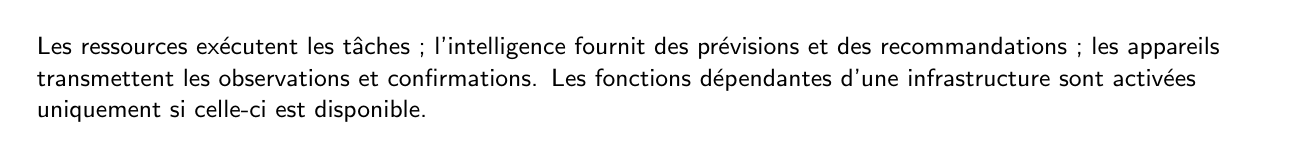
\begin{tikzpicture}[x=1cm,y=-1cm]
\pband{0}{RESSOURCES ET INFRASTRUCTURES}{Green}
\pblock{0}{.35}{5.1}{4.05}{Green}{Gestion de la main-d’œuvre}{Planification du personnel\par Suivi des performances\par Gestion des compétences\par Équilibrage de la charge\par Suivi de la productivité}
\pblock{5.45}{.35}{5.1}{4.05}{Green}{Gestion des équipements}{Chariots et transpalettes\par Convoyeurs et trieurs\par AS/RS et navettes\par AMR, AGV et robots\par Maintenance}
\pblock{10.9}{.35}{5.1}{4.05}{Green}{Énergie et environnement}{Consommation par zone\par Consommation des équipements\par Température et humidité\par Seuils et consignes\par Marche, veille et arrêt\par Pics de consommation\par Historique énergétique}
\pblock{0}{4.7}{7.8}{3.35}{Green}{Interfaces WCS / WES}{Instructions aux équipements\par État des équipements et gestion des erreurs\par Contrôle des itinéraires\par Gestion du trafic et des tâches}
\pblock{8.2}{4.7}{7.8}{3.35}{Green}{Gestion des actifs}{Suivi des actifs\par Étalonnage et taux d’utilisation\par Surveillance de l’état\par Gestion du cycle de vie}
\pband{8.6}{INTELLIGENCE ET AIDE À LA DÉCISION}{Purple}
\pblock{0}{8.95}{5.1}{3.1}{Purple}{Prévision de la demande et de la charge}{Prévisions des flux entrants\par Prévisions des flux sortants\par Prévisions des besoins\par en ressources}
\pblock{5.45}{8.95}{5.1}{3.1}{Purple}{Optimisation du slotting}{Classement ABC et rotation\par Occupation de l’espace\par Règles dynamiques\par de placement}
\pblock{10.9}{8.95}{5.1}{3.1}{Purple}{Optimisation des ordres et tâches}{Regroupement des vagues\par Optimisation des parcours\par Séquencement des tâches\par Priorisation intelligente}
\pblock{0}{12.35}{7.8}{2.9}{Purple}{Optimisation de la main-d’œuvre}{Niveaux d’effectifs\par Affectation des tâches\par Productivité et équilibrage de la charge}
\pblock{8.2}{12.35}{7.8}{2.9}{Purple}{Anomalies et risques}{Détection d’anomalies\par Écarts de processus et gestion des risques\par Tableaux de contrôle}
\pband{15.8}{TERMINAUX ET APPAREILS DE TERRAIN}{Teal}
\pblock{0}{16.15}{7.8}{3.3}{Teal}{Identification et observation}{Terminaux RF\par Scanners codes-barres / QR\par Lecteurs RFID\par Caméras / vision\par Capteurs}
\pblock{8.2}{16.15}{7.8}{3.3}{Teal}{Mesure, guidage et confirmation}{Balances et pesage\par Systèmes vocaux\par Smartphones et tablettes\par Pick-to-Light / Put-to-Light\par Terminaux embarqués}
\node[anchor=north west,text width=15.6cm,font=\sffamily\fontsize{9}{11.5}\selectfont] at (0,19.8) {Les ressources exécutent les tâches ; l’intelligence fournit des prévisions et des recommandations ; les appareils transmettent les observations et confirmations. Les fonctions dépendantes d’une infrastructure sont activées uniquement si celle-ci est disponible.};
\end{tikzpicture}
